%\section{Einleitung}
\subsection{Callback}
\begin{frame}
  \frametitle{Callback}
  \framesubtitle{Idee}
  \begin{itemize}
    \item Funktion (Methode oder Prozedur) als Argument an eine andere Funktion
    \item Nach Abschluss einer bestimmten Aufgabe wird Funktion ausgeführt
    \item Aufrufende Funktion muss nichts vom Callback wissen
    \item Kommunikation unidirektional
    \item Callback-Pattern wird häufig in der asynchronen Programmierung verwendet
    \item Callback-Pattern eignet sich gut für ereignisgesteuerte Programmierung
  \end{itemize}
\end{frame}

\begin{frame}
  \frametitle{Callback}
  \framesubtitle{Callback Pattern}
  \begin{figure}[!ht]
    \centering
    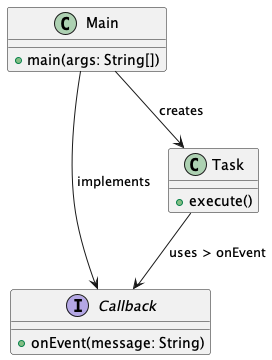
\includegraphics[width=0.35\textwidth]{fig/uml/callback-class.png}
    \caption{Callback Pattern}
    \label{fig:callback-class}
  \end{figure}
\end{frame}

\begin{frame}
  \frametitle{Callback}
  \framesubtitle{Callback Pattern Sequenz}
  \begin{figure}[!ht]
    \centering
    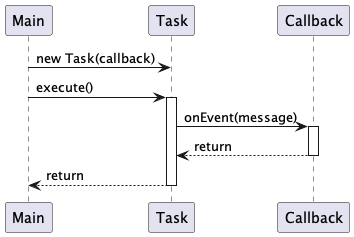
\includegraphics[width=0.65\textwidth]{fig/uml/callback-seq.png}
    \caption{Callback Pattern Sequenz}
    \label{fig:callback-seq}
  \end{figure}
\end{frame}
